\documentclass[
	12pt,
	openright,
	twoside,
	a4paper,
	oneside,
	brazil,
	chapter=TITLE,
	%section=TITLE,
	%subsection=TITLE,
	sumario = tradicional
]{abntex2}

\usepackage[font=small,format=plain,labelfont=bf,up,margin=1cm]{caption}
\usepackage{amsmath}
\usepackage[utf8]{inputenc}
\usepackage[T1]{fontenc}
\usepackage[pdftex]{graphicx}
\usepackage{subfig}
\usepackage{float}
\usepackage[alf,abnt-etal-list=0, abnt-etal-cite=2, abnt-etal-text=it, abnt-repeated-author-omit=yes, abnt-emphasize=bf]{abntex2cite}
% alf - exibi as referencias em ordem alfabetica.
% abnt-etal-list=0 - foi utilizado para não permitir o uso de et al. nas referências.
% abnt-etal-cite=2 - mostra que pode ser feita a citação de até 2 autores no texto. Se numa referência existem 3 autores, usa-se evidentemente o et al., com a citação do primeiro autor.
% abnt-etal-text=it - exibi a escrita do et al nas referencias em italico.
\usepackage{svg}
\usepackage{indentfirst} % justificar automaticamente os parágrafos
\usepackage{lscape}
\usepackage{import}
\usepackage{helvet}
\renewcommand{\familydefault}{\sfdefault}
\usepackage{lastpage}			% Usado pela Ficha catalográfica
\usepackage{color}				% Controle das cores
\usepackage{microtype} 			% para melhorias de justificação

%unidades de medida em equações
\usepackage{siunitx}
\sisetup{detect-all}
%%%%%%%%%%%%%%%%%%%%%%

% Acrescentado para gerar as tabelas 22/07/2017
\usepackage[normalem]{ulem}
\useunder{\uline}{\ul}{}

\usepackage{longtable}
\usepackage{empheq}
\usepackage{multirow}
\usepackage{booktabs}
\usepackage{pdfpages} %adicionar pdfs


\newcommand*\widefbox[1]{\fbox{\hspace{2em}#1\hspace{2em}}}
\newcommand{\head}[1]{\textnormal{\textbf{#1}}}
\newcolumntype{C}[2]{>{\centering\vspace{#2}\let\newline\\\arraybackslash\hspace{0pt}\vspace{#2}}m{#1}}

% Préambulo --------------------------------------------------------------------------------------------------------------------------

\newcommand{\universidade}{Universidade Federal do Vale do São Francisco }
\newcommand{\curso}{Engenharia Elétrica}
\newcommand{\graduacao}{Curso de Graduação em \curso}
\newcommand{\bancaum}{Prof. Dr. Rodrigo Pereira Ramos (CENEL)}
\newcommand{\bancadois}{Prof. Dr. José Bismark de Medeiros (CEMEC)}
\newcommand{\bibliotecario}{Inserir Bibliotecário}
\newcommand{\cpf}{052.376.974-19}

\autor{Daniel Simião Nunes Oliveira}

% altera o tamanho da assinatura
\setlength{\ABNTEXsignwidth}{9cm}

%\titulo{Geração de Energia Elétrica com Biogás de Aterro Sanitário: Um Mecanismo de Desenvolvimento Limpo para Petrolina - PE}
\titulo{Análise da Geração de Energia Elétrica com Biogás no Aterro Sanitário de Petrolina - PE}
\tipotrabalho{Trabalho de Conclusão de Curso}
\orientador[Orientador:]{Prof. Dr. Eduard Montgomery Meira Costa}
%\coorientador[Coorientador: Dr.]{Brauliro Gonçalves Leal}
\instituicao{\universidade \par \curso}
\local{Juazeiro - BA}
\data{2019}
\preambulo{
	Trabalho de Conclusão de Curso apresentado como requisito parcial para obtenção do título de Bacharel em \curso, pela \universidade - UNIVASF.
}

% alterando o aspecto da cor azul.
\definecolor{blue}{RGB}{41,5,195}

% Configurações de aparência do PDF final.
\makeatletter

%%%%%%%%% unidades de medida equações
\providecommand\add@text{}
\newcommand\tagaddtext[1]{%
  \gdef\add@text{#1\gdef\add@text{}}}% 
\renewcommand\tagform@[1]{%
  \maketag@@@{\llap{\add@text\quad}(\ignorespaces#1\unskip\@@italiccorr)}%
}
%%%%%%%%%%%%%%%%%%%%%%%%%%%%%

\long\def\ifnodedefined#1#2#3{%
    \@ifundefined{pgf@sh@ns@#1}{#3}{#2}%
}
\hypersetup {
    breaklinks      = true,
	pdftitle		= {\@title},
	pdfauthor		= {\@author},
	pdfsubject      = {\imprimirpreambulo},
	pdfcreator		= {LaTeX com abnTeX2},
	pdfkeywords 	= {Geração Distribuída}{Biogás}{Biometano}{Aterro Sanitário},
	colorlinks		= true,			% false: boxed links; true: colored links
	linkcolor		= black,         % cor links internos.
	citecolor		= black,       	% cor links referencias bibliograficas.
	filecolor		= magenta,		% cor links de arquivos.
	urlcolor		= black,			% Cor url.
	bookmarksdepth	= 4
}

%escrever subescrito
\usepackage{fixltx2e}

%%%%%%%%%%%%%%
\makeatother

% compila o sumário
\makeindex  



% Altera as margens padrões
\pagenumbering{arabic}

%pacotes para desenhos e gráficos
\usepackage{tikz}
\usepackage{pgfplots}

% Espaçamentos  entre linhas e parágrafos 
% O tamanho do parágrafo é dado por:
\setlength{\parindent}{1.5cm}
% Controle do espaçamento entre um parágrafo e outro:
\setlength{\parskip}{0.2cm}  % tente também \onelineskip



% Retira espaço extra obsoleto entre as frases.
\frenchspacing


\usepackage{leftidx}

\begin{document}

	\renewcommand{\imprimircapa} {
	\begin{capa}
		\center

		\vspace*{-2.5cm}

		\begin{figure}[!htbp]
		 	\centering
		 	
\includegraphics[scale=0.08]{./figuras/univasf.pdf}
		\end{figure}

		\ABNTEXchapterfont {\large \textbf {\MakeUppercase{\universidade}\\ \MakeUppercase{\graduacao} }}

		\vspace*{3cm}

		\ABNTEXchapterfont {\MakeUppercase{\Large \imprimirautor}}

		\vfill

		\begin{center}
			\ABNTEXchapterfont \bfseries {\LARGE \imprimirtitulo}
		\end{center}

		\vfill

		{\large \imprimirlocal} \\
		{\large \imprimirdata}

		\vspace*{1cm}
	\end{capa}
}
	\makeatletter
\renewcommand{\folhaderostocontent} {
	\begin{center}
		\ABNTEXchapterfont {\large \textbf {\MakeUppercase{\universidade}\\ \MakeUppercase{\graduacao} }}
		\vspace*
		\fill

		{\ABNTEXchapterfont\MakeUppercase{\Large\imprimirautor}}

		\vspace*{\fill}

		\begin{center}
			{\ABNTEXchapterfont\bfseries\LARGE\imprimirtitulo}
		\end{center}

		\vspace*{\fill}\vspace*{\fill}

		\abntex@ifnotempty{\imprimirpreambulo} {
			\hspace{.45\textwidth}
			\begin{minipage}{.5\textwidth}
				\SingleSpacing
				\imprimirpreambulo \\\\
				\imprimirorientadorRotulo~\imprimirorientador\\
				\imprimircoorientadorRotulo~\imprimircoorientador
			\end{minipage}
			\vspace*{\fill}
		}

		\vspace*{\fill}\vspace*{\fill}

		{\large\imprimirlocal}
		\par
		{\large\imprimirdata}
	\end{center}

	\newpage
}
\makeatother
	\newcommand{\imprimirdedicatoria} {
	\begin{dedicatoria}
		\vspace*{\fill}
			\begin{flushright}
				\textit {
					Dedico esse trabalho a minha mãe Maria José (in memorian), com todo o meu amor, gratidão e saudades.
						}
			\end{flushright}
	\end{dedicatoria}
}
	\newcommand{\imprimiragradecimentos}{
\begin{agradecimentos}
    \noindent Agradeço aos meus pais José Neuton Alves de Oliveira e Maria José Nunes de Oliveira pela perseverança, insistência e fé.
\end{agradecimentos}
}

	\newcommand{\imprimirepigrafe} {
	\begin{epigrafe}
		\vspace*{\fill}
		\begin{flushright}
			\textit {
				''Meu sonho não tem fim e nada vai me afastar do amor de Deus'' (Ayrton Senna)
			}
		\end{flushright}
	\end{epigrafe}
}
	
\newcommand{\imprimirresumo} {
\setlength{\absparsep}{18pt} % ajusta o espaçamento dos parágrafos do resumo

\begin{resumo}
resumo

    \noindent\textbf{Palavras-chaves}: Aterro Sanitário; Biogás; Geração Distribuída; Energia Elétrica e Retorno Financeiro.
\end{resumo}

% --- resumo em inglês ---
\begin{resumo}[Abstract]
	\begin{otherlanguage*}{english}

Abstract

\noindent\textbf{Keys}: Landfill; Biomethane; Distributed Generation; Eletricity Generation and Payback.
	\end{otherlanguage*}
\end{resumo}
}
	\newcommand{\imprimirabreviaturas} {
	\begin{siglas}
		\item[ANEEL] Agência Nacional de Energia Elétrica
		\item[BNDES] Banco Nacional de Desenvolvimento Econômico e Social
		\item[TTE] Contribuição para o Financiamento da Seguridade Social
		\item[EE] Eficiência Energética
        \item[EPE] Empresa de Pesquisa Energética
		\item[GD] Geração Distribuída
		\item[GMG] Grupo Moto Gerador
		\item[GEE] Gases de Efeito Estufa
		\item[ICMS] Imposto sobre Circulação de Mercadorias e Serviços
		\item[IBGE] Instituto Brasileiro Geografia e Estatística
		\item[INPE] Instituto Nacional de Pesquisas Espaciais
		\item[MDL] Mecanismo de Desenvolvimento Limpo
		\item[MME] Ministério de Minas e Energia
		\item[ONU] Organização das Nações Unidas
		\item[PIS] Programa de Integração Social
		\item[PRODIST] Procedimentos de Distribuição de Energia Elétrica no Sistema Elétrico Nacional
		\item[REN] Resolução Normativa	
		\item[SEB] Sistema Elétrico Brasileiro
		\item[SIN] Sistema Interligado Nacional
		\item[TUST] Tarifa de Uso dos Sistemas de Transmissão
		\item[TUSD] Tarifa de Uso dos Sistemas de Distribuição
		\item[UNFCCC] United Nations Climate Change
	\end{siglas}
}



	\selectlanguage{brazil}

	% ELEMENTOS PRE-TEXTUAIS

	\pretextual

	% Capa
	\imprimircapa
	
	% Folha de Rosto
	\folhaderostocontent
	
	% Ficha Catalográfica	
	%\input{elementos-pretextuais/fichacatalografica.tex}
	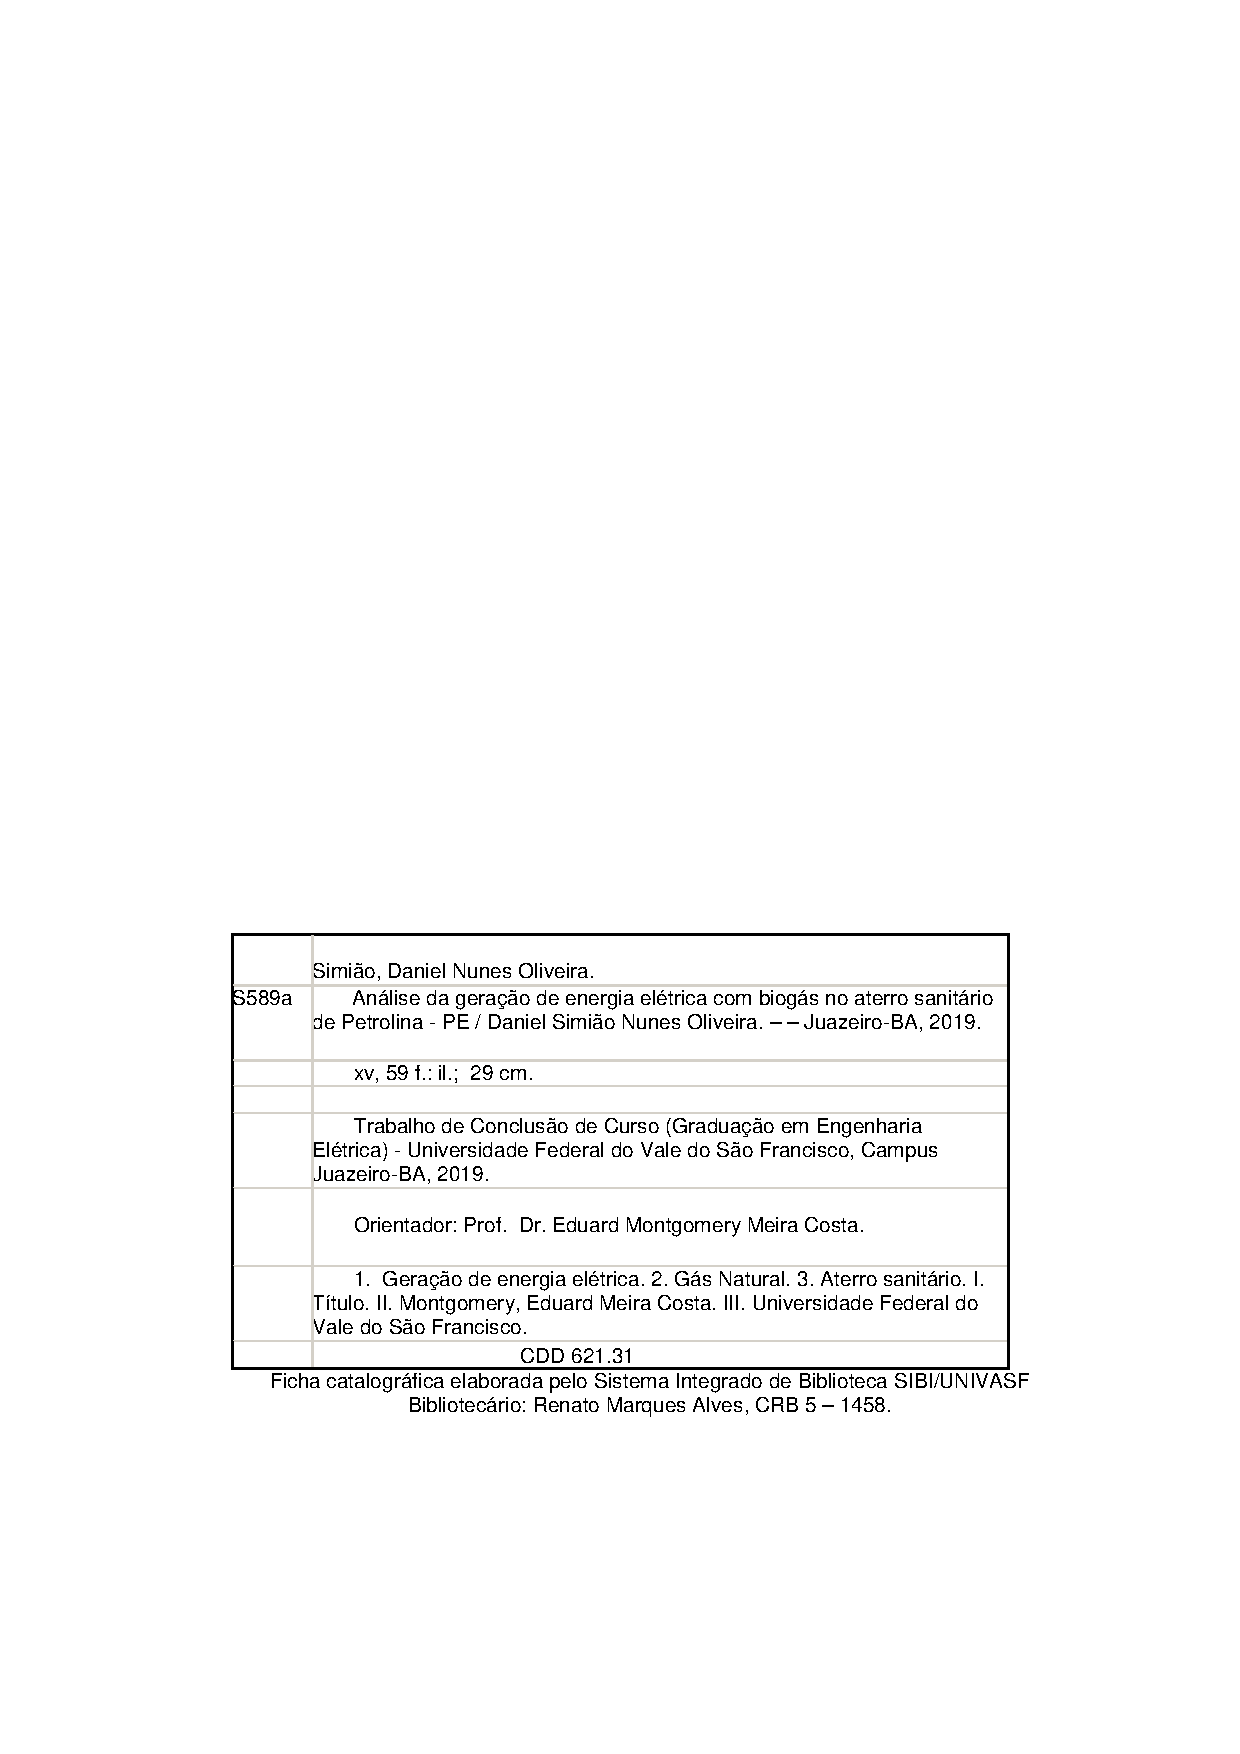
\includepdf[pages=-]{Digitalizado/ficha.pdf}
	%Parecer da Banca
    \newpage

\vspace*{-2.5cm}

\begin{figure}[!htbp]
 	\centering
 	
\includegraphics[width=3cm]{./figuras/brasao.pdf}\\
 	\small{\textbf{SERVIÇO PÚBLICO FEDERAL MINISTÉRIO DA EDUCAÇÃO}}\\
	\textbf{SECRETARIA DE EDUCAÇÃO SUPERIOR}
\end{figure}

\begin{center}
    \ABNTEXchapterfont {\textbf {\MakeUppercase{\universidade}\\ \MakeUppercase{\graduacao} }}
\end{center}

\vspace{1cm}

\begin{center}
    \MakeUppercase{Parecer da banca examinadora de defesa de trabalho de conclusão de curso}
\end{center}

\vspace{1cm}

\begin{center}
    \emph{\Large\imprimirautor}
\end{center}


\noindent A Banca Examinadora composta por: \emph{\imprimirorientador}, \emph{\bancaum} e pelo \emph{\bancadois} consideram o candidato \textbf{APROVADO} com nota \textbf{9,0}.

\vspace{1cm}

\begin{center}
    Juazeiro - BA, 27 de Março de 2019.
\end{center}

\begin{center}
	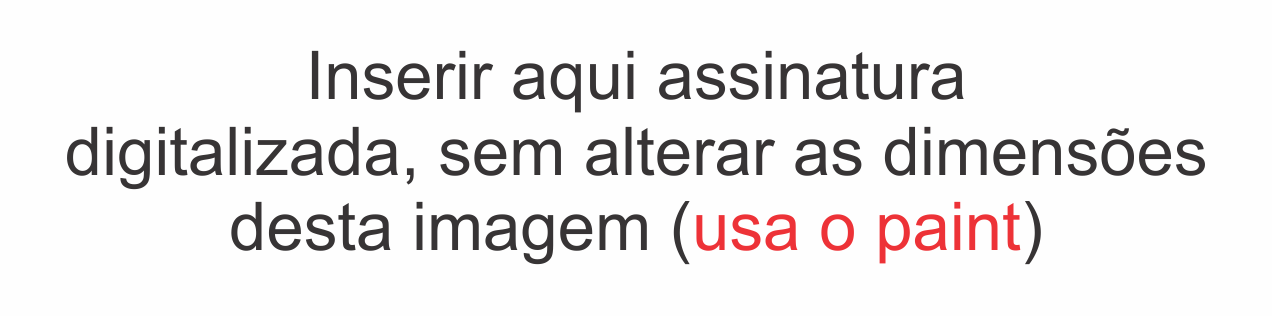
\includegraphics[scale=1]{Digitalizado/assinaturaOrientador.png}\\
	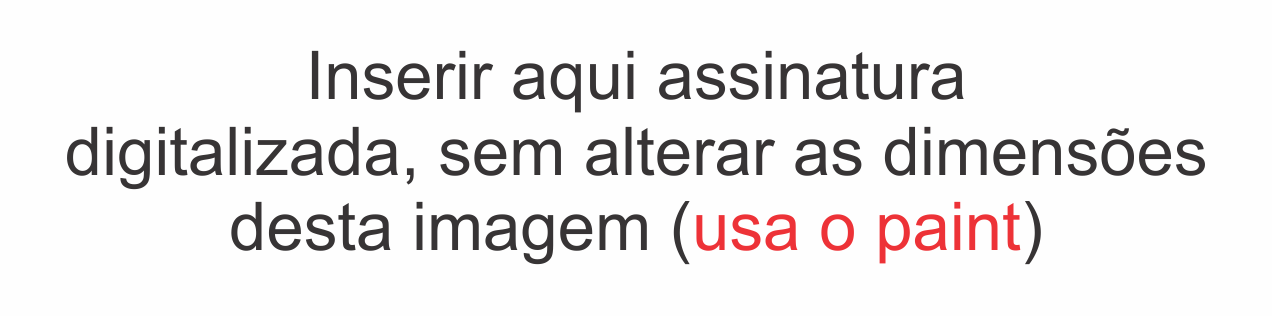
\includegraphics[scale=1]{Digitalizado/assinaturaAvaliador01.png}\\
	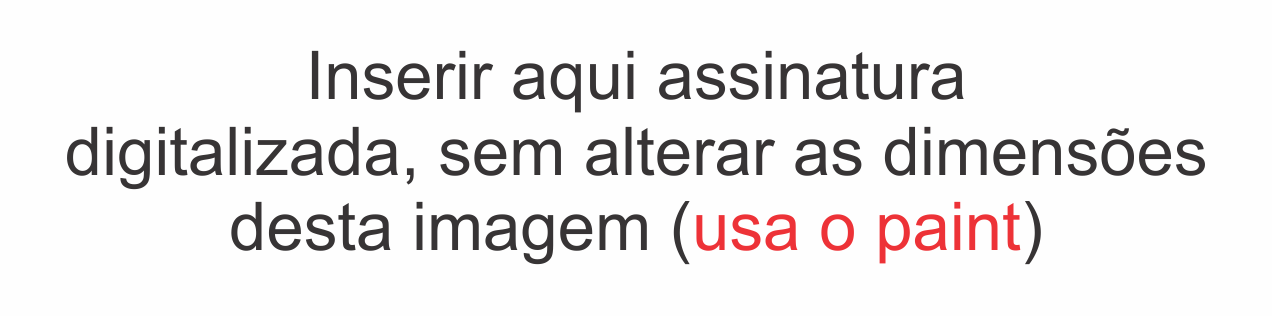
\includegraphics[scale=1]{Digitalizado/assinaturaAvaliador02.png}
\end{center}

\newpage
	%Declaração de Conformidade
    \chapter*{Declaração de Conformidade}

\noindent Eu, \MakeUppercase{\textbf{\imprimirautor}}, declaro que este Trabalho de Conclusão de Curso (TCC) intitulado:

\begin{center}
    \MakeUppercase{\textbf{\imprimirtitulo}}
\end{center}

\noindent é de minha autoria e confirmo que:

\begin{enumerate}
    \item Nenhuma parte deste trabalho foi submetida a nenhum tipo de avaliação de qualificação nesta ou em qualquer outra Universidade;

    \item Todas as \textit{obras, artigos e/ou divulgações}, de qualquer natureza, de outros autores ou de co-autoria utilizadas para elaboração deste trabalho têm seus créditos devidamente atribuídos;

    \item A versão denominada \textbf{versão final}, contém as solicitações de correção exigidas pela Banca Examinadora por ocasião da defesa deste trabalho, e atende as normas contidas no Manual de Normatização de Trabalhos Acadêmicos da UNIVASF em vigor.
\end{enumerate}

\vspace{1cm}

\begin{center}
    Juazeiro - BA, 27 de março de 2019.
\end{center}

\begin{center}
	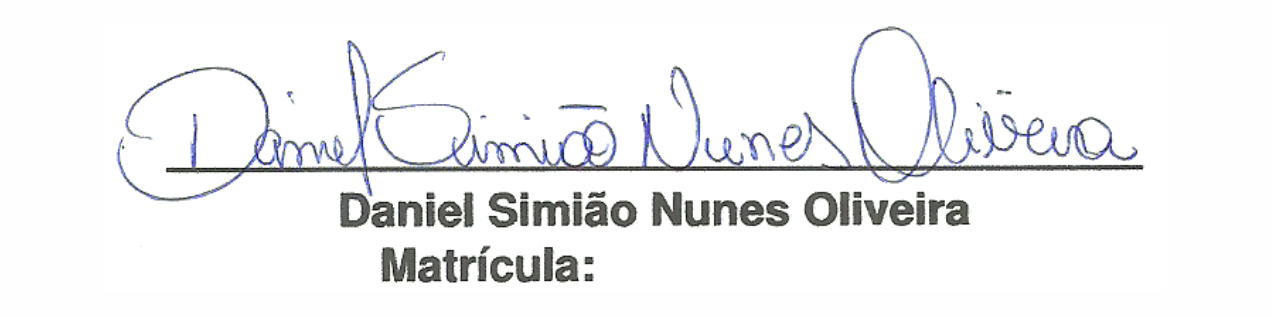
\includegraphics[scale=1]{Digitalizado/assinaturaAluno.png}
\end{center}

\newpage

	% Folha de Aprovação
	%\begin{folhadeaprovacao}
		\begin{center}
			{\ABNTEXchapterfont \large \textbf {\MakeUppercase{\universidade}\\ \MakeUppercase{\graduacao} }}

			\vspace*{22pt}

			FOLHA DE APROVAÇÃO %\\ Para TCC

			\vspace*{30pt} %\vspace*{\fill}

			{\ABNTEXchapterfont\Large\imprimirautor}

			\vspace*{18pt}

			\begin{center}
				{\ABNTEXchapterfont\Large\imprimirtitulo}
			\end{center}

			\vspace*{40pt} %\vspace*{\fill}

			\imprimirpreambulo
		\end{center}

		\assinatura{\imprimirorientador\\ \universidade}
		\assinatura{\bancaum}
		\assinatura{\bancadois}

		\vspace*{77pt} %\vspace*{\fill}
		Aprovado pelo Colegiado de Engenharia Elétrica em 27 de Março de 2019.
\end{folhadeaprovacao}

    
	% Dedicatoria
	\imprimirdedicatoria
	
	% Incluindo os agradecimentos
	\imprimiragradecimentos
	
	% Epigrafe
	\imprimirepigrafe
	
	% Resumo e Abstract
	\imprimirresumo

	% Lista de Abreviaturas
	\imprimirabreviaturas
	
	% Lista de Figuras
	
	\renewcommand*\listfigurename{Lista de Figuras}
	\listoffigures*
	\cleardoublepage	
	
	% Lista de Tabelas
	\renewcommand*\listtablename{Lista de Tabelas}
	\listoftables*
	\cleardoublepage


	% Índice (Sumário)
	\tableofcontents*
	\cleardoublepage
	
	%%%%%%%%%%%%%%%%%%% ELEMENTOS TEXTUAIS %%%%%%%%%%%%%%%%
	\chapterstyle{BlackBox}
	\textual
	%\pagestyle{simple}
	
	% Inserir meus capítulos aqui
	
	%introdução
	\chapter{Introdução}



\section{Motivação}


O posicionamento social está mudando e junto com ele a forma de consumir produtos e serviços sustentáveis. Esta postura, contribui para a preservação do planeta, uma vez que os recursos renováveis são limitados, forçando a humanidade trilhar um caminho mais consciente e harmonioso com a natureza. Assim, o interesse em discorrer sobre a geração de eletricidade utilizando o biogás do aterro sanitário, surgiu a partir da necessidade de desenvolver projetos sustentáveis com foco na geração de energia limpa. 


\section{Justificativa}

Diante dessa problemática, surgiu o seguinte questionamento: como gerar energia elétrica utilizando os resíduos sólidos, transformando o lixo de passivo ambiental para ativo financeiro.

Petrolina (PE) está inserida no mercado internacional, com foco no escoamento da produção agrícola. Atualmente, é cada vez mais comum os consumidores estrangeiros buscarem informações completas que permitem o rastreio da cadeia produtiva de um alimento, dispondo de dados da colheita, adubação e impactos ambientais \cite{europa}. Assim, a busca por informações que dizem a real origem dos alimentos tem crescido nos últimos anos, principalmente aqueles que serão colocados na mesa do consumidor europeu. 

Esta situação evidencia a forte tendência global não só pela forma como são produzidos os alimentos, mas de onde eles vêm e sua influência socioeconômica. Uma pesquisa realizada em Bruxelas, pela Organização Europeia do Consumidor (BEUC), revelou que 70\% das pessoas entrevistadas afirmaram que conhecer a origem da comida é um fator crucial para determinar as compras no supermercado, principalmente daqueles itens consumidos diariamente \cite[pág. 6]{beuc:consumo}. Tal cenário sinaliza com luz amarela a necessidade de investir em empreendimentos que promovam a redução dos gases de efeito estufa (GEE).

As mudanças climáticas forçaram os governos a planejarem incentivos fiscais e subsídios financeiros para as fontes renováveis. São ações que proporcionam uma política de diversificação das matrizes energéticas e, consequentemente, o amadurecimento tecnológico das indústrias de energia solar, eólica e de biogás. O projeto de lei do Senado Federal nº 712/2015 aumenta a participação das energias renováveis na matriz energética em pelo menos 60\% até 2040. %desfecho

A Portaria nº 65 do Ministério de Minas e Energia (MME), publicada no dia 28 de fevereiro de 2018, no Diário Oficial da União, determinou um Valor Anual de Referência Específico (VRES) para a biomassa dedicada de R\$ 537,00 e gás natural a um custo de R\$ 451,00 por MWh. A valorização do MWh para fornecimento de eletricidade, com energias renováveis, representa um cenário muito atrativo para investimento em usinas termoelétricas que utilizam o biogás como combustível.


\section{Objetivo Geral}
Identificar a viabilidade econômica da construção de uma usina termoelétrica, localizada no aterro sanitário de Petrolina (PE), aproveitando o biogás gerado pelo lixo em decomposição.


\section{Objetivos Específicos}

\begin{itemize}
    \item Analisar o tempo de vida útil e a capacidade de produção de energia elétrica do aterro sanitário;
    \item Identificar o perfil financeiro e o consumo de energia elétrica do município ao longo do ano de 2018;
    \item Avaliar o tempo de retorno do investimento e ganhos financeiros para a administração pública.
\end{itemize}

\section{A Relevância do Trabalho}
O presente trabalho é importante porque promove exploração energética do metano que é produzido pelo aterro sanitário. Bem como, é uma atividade econômica inexplorada na região, cenário que condiciona a evolução ou criação de empresas locais voltadas para o reaproveitamento energético do lixo urbano.

\section{Organização do Trabalho}
Este trabalho é composto por cinco capítulos, os quais são descritos a seguir:

\begin{itemize}
    \item No Capítulo 2, são apresentados os fundamentos teóricos quanto às formas de produção, conversão e transmissão de energia, além da estruturação do sistema elétrico brasileiro voltado para o biometano, uma evolução no aproveitamento das fontes renováveis ante o uso de combustíveis fósseis;
    \item No Capítulo 3, apresenta-se uma visão micro e macroeconômica da cidade de Petrolina (PE) no contexto da globalização;
    \item No Capítulo 4, descreve-se a metodologia utilizada para projetar uma usina termelétrica em minigeração distribuída, considerando a localização e potência desejada
    \item No Capítulo 5, são apresentados os resultados pertinentes à rentabilidade, financiamento, compensação ou venda da eletricidade, a fim de comprovar a viabilidade econômica do empreendimento;
    \item No Capítulo 6, são realizadas as considerações finais, focalizando as reflexões sobre a geração de energia elétrica com biogás no aterro sanitário de Petrolina (PE).
\end{itemize}

	
	%fundamentação teórica
	\chapter{Fundamentação Teórica}

Desenvolver a fundamentação teórica


	
	%metodologia
	\chapter{Metodologia}

Inserir metodologia utilizada aqui

	
	%resultados e discussões
	\chapter{Resultados e Discussões}

Inserir resultados e discussões dos resultados
	
	%conclusão
	\chapter{Conclusão}

Inserir conclusão
	



	%%%%%%%%%%% ELEMENTOS POS-TEXTUAIS %%%%%%%%%%%
	\postextual

	\chapterstyle{abnt}

	\bibliographystyle{abntex2-alf}
	\bibliography{referencias}

%para inserir ou remover apendices e anexos, basta adicionar ou remover o percentual (comentário %) 	
 	%%Apêndice
\appendix

\begin{apendicesenv} %inicio dos apendices
	\partapendices
	\chapter{Título}
	
	Inserir apendices
	
\end{apendicesenv}%fim dos apendices
	%\begin{anexosenv} % início dos anexos

% Imprime uma página indicando o início dos anexos
\partanexos

\chapter{Título}

Inserir anexos se houver


\end{anexosenv} % fim dos anexos
	

\end{document}
